
\section{Research Direction: Testing and Troubleshooting}
\label{sec:testing-debugging}

\subsection{Software Testing as a Service}

Within the increasing demand for software development as a service,
\textit{software testing as a service} has seen significant growth and adoption
in its own right, often as a separate service that is independent of development
activities. In fact, according to a 2006 survey,\footnote{\scriptsize
  \url{http://www.drdobbs.com/architecture-and-design/cheapers-not-always-better/184415486?requestid=247829}}
software testing was the second largest outsourced software-engineering activity
after coding: 81\% of the 200 industrial practitioners, who participated in the
survey, stated that they outsource software testing. Given this trend, services
companies now routinely offer services that focus exclusively on testing
activities.

%% The engagement modes can vary: staff augmentation, core/flex, managed service
%% (fixed capacity, outcome based). But perhaps this needs to be mentioned earlier
%% as these modes are not particular to testing services.

\begin{figure}[t]
\centering
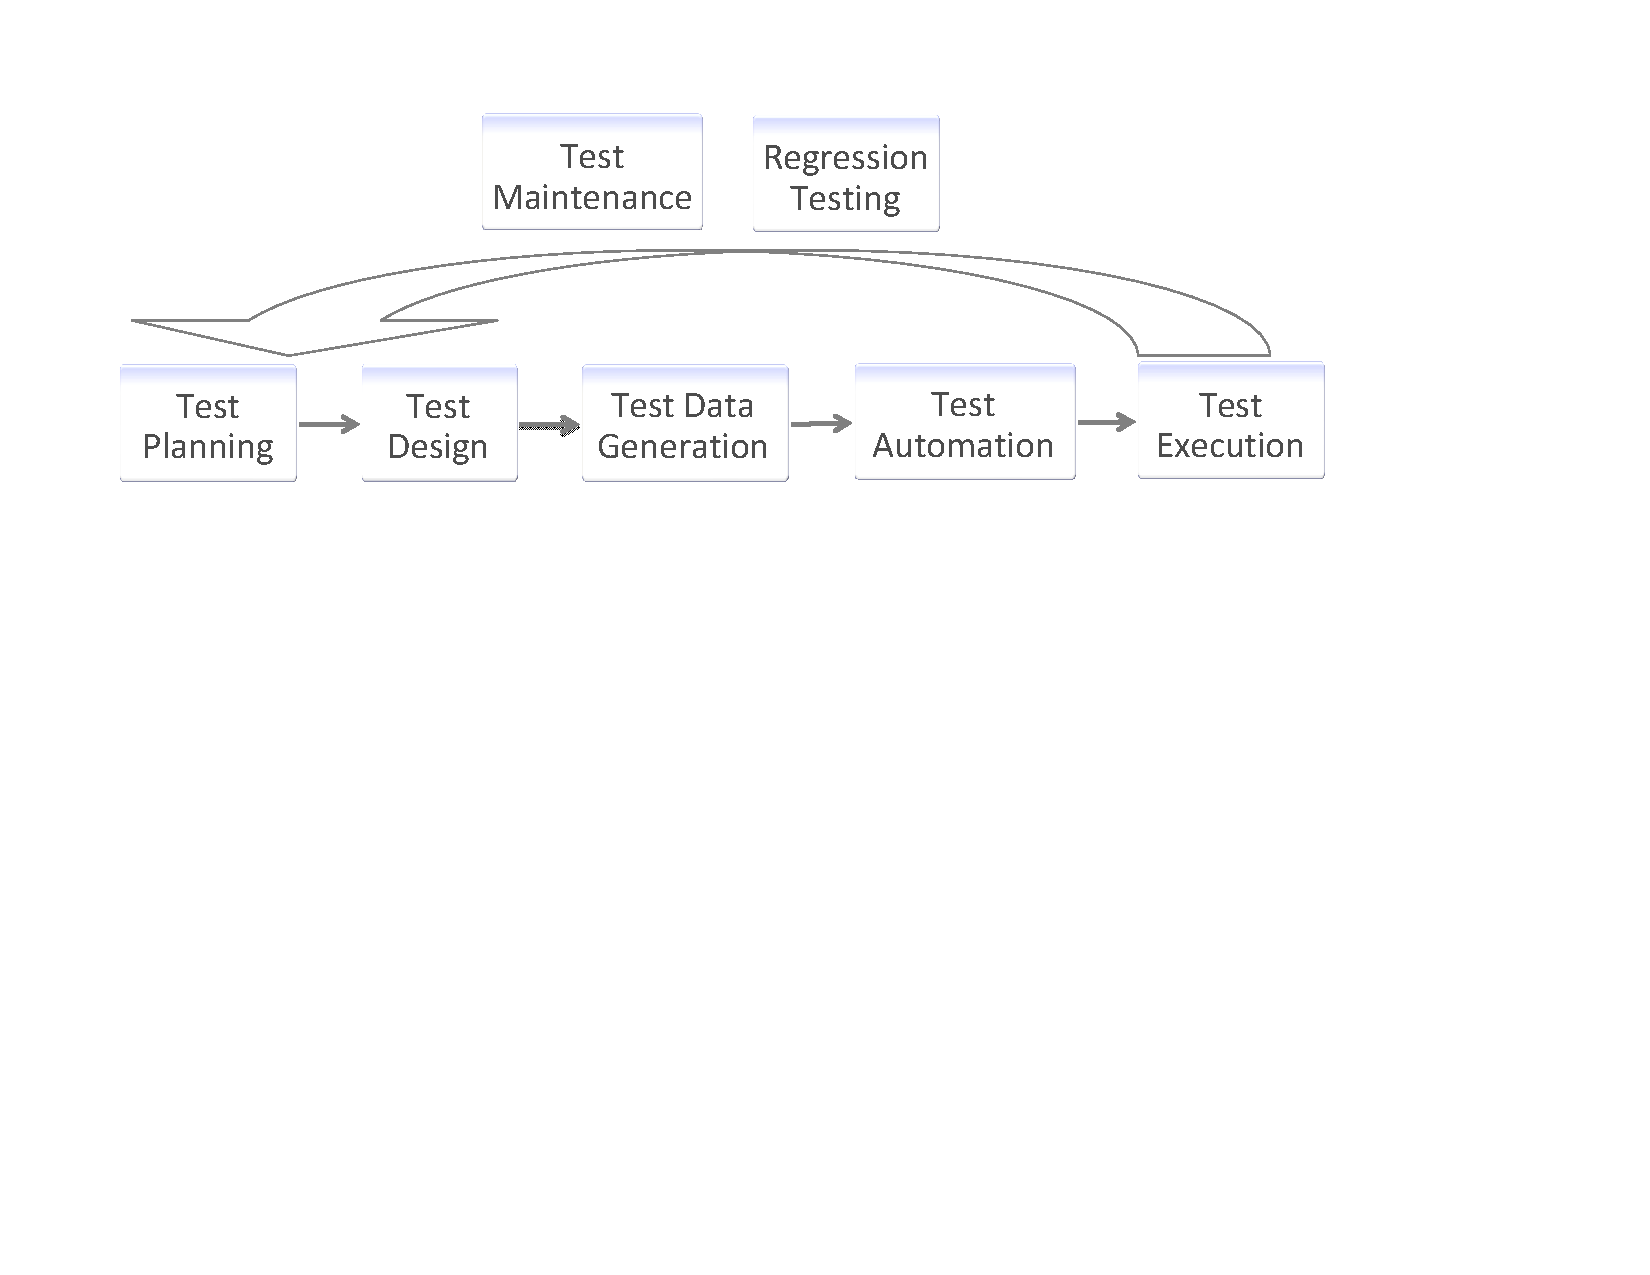
\includegraphics[width=\columnwidth, clip, trim = 20mm 133mm 55mm
  18mm]{figs/testing-activities.pdf}
\vspace*{-15pt}
\caption{Typical testing activities performed in delivery of testing services.}
\vspace*{-10pt}
\label{fig:testing-activities}
\end{figure}

The nature of the activities performed in a testing-services engagement can vary
from client to client; but, typically, the scope of work includes activities,
such as test design, test-data creation, test automation, test execution, and
test maintenance. Figure~\ref{fig:testing-activities} presents an overview of
the commonly performed activities in the delivery of testing services. A
delivery engagement might involve any subset of these activities. For example,
delivery for a client might involve only manual test execution, or the scope of
work may include test automation and test maintenance as well. In other cases,
the scope of work may be even broader, encompassing test design and/or test
planning. The nature of the test cases can also vary from functional tests to
tests that focus on validating non-functional system properties, such as
performance and security.

The activities shown in Figure~\ref{fig:testing-activities}, of course, pertain
to testing in general (whether performed in-house or in an outsourced manner),
but there are factors that can add unique challenges in the setting of testing
services. For instance, many of these activities can require specific skills in
testing techniques/tools or coding expertise, which the average testing
practitioner involved in service delivery may not possess. Second, some of the
activities may need to be carried out in strict time-bound cycles and
client-controlled test environments. Finally, the myriad of technologies that
must be accommodated in the contexts of the IT systems of different clients adds
another layer of complexity for service companies.

\subsubsection{Test Planning}
\label{sec:test-planning}

\subsubsection{Test Design}
\label{sec:test-design}

Optimization of test cases using techniques such as combinatorial test design.

\subsubsection{Test Data Generation}
\label{sec:test-data}

\subsection{Test Data Generation}

Enterprise applications are typically database-oriented, in that they make queries over databases and the program flow depends on the data retrieved as a result of a query.  In order to test whether the application satisfies its requirements, sufficient amount of test data must be made available in the database. Consider, for example, a banking application, in which one of the requirement to exercise is that if a customer makes a certain fixed deposit, and the person is a senior citizen, and also holds a checking account in the bank, then an addition 0.25\% is paid as interest. To test that this situation is handled correctly in the application, there should exist a customer in the database such that his or her age qualifies the person as senior citizen and the person also has a checking account. Notice that typically, customer data and account data would be maintained in separate database tables. Typically business requirements are complex, and there need to be specific entries in multiple tables for a scenario to work out.

When a client gives a testing contract, the client may expect the service provider to exercise all the business rules, but may not give enough sample data in the database to be able to exercise these rules.  It then becomes the responsibility of the service provider to figure out the requisite test data to be present in the pertinent tables.

Randomly generated test data  cannot be expected to suffice for enterprise applications with complex rules. Also, systematic test generation approaches based on program analysis cannot be expected to tackle enterprise application, which use a mix of multiple language and database technologies in their implementation. The database community has done some work in creating test data for SQL queries, and that may be relevant; however, as mentioned before, enterprise applications are implemented with a mix of technologies.

We see a big opportunity for research contributions in this subarea. How to take a specification of the application as testing criteria, and automatically populate database that would enable various scenarios that fulfill the test criteria to be exercised.


\subsubsection{Test Automation}
\label{sec:test-automation}

The functional test cases created during test design are often stated informally
in natural language. These tests are known as \textit{manual test cases}, which
consist of a sequence of steps, intended for execution by a human on the
application user interface.  Test automation is the activity of converting these
test cases into test scripts or programs that perform the test steps
mechanically.

Although test automation is desirable (\eg for efficient and predictable test
executions) and sometimes necessary (\eg to meet time-constrained regression
schedules), creating \textit{robust} test scripts that can be used repeatedly in
regression cycles is expensive. In essence, creating such scripts is
time-consuming, involving a significant amount of coding, and requires expertise
in test automation tools (\eg \cite{hpqtp,ibmrft,selenium}). In the context of
service delivery, this poses the unique challenge: how can change-resilient test
automation be performed efficiently by delivery personnel who may not possess
good programming skills or deep tool knowledge?

Moreover, test automation involves not only the one-time cost of creating the
scripts, but also a recurring cost of maintaining the scripts in response to
application changes and changes in the execution environment.

No one technique of UI element identification is likely to be the best in all
circumstances; therefore, the choice of the technique needs to be based on the
requirements for testing (e.g., execution of scripts across browsers, across
internationalized variants of application, etc.)

Cross-browser testing: keeping up with browser upgrades, reduce reliance on DOM
structure and attributes.

Relate to program synthesis: (1) basic generation of change-resilient method of
identifying a UI element; (2) synthesis of custom functions based on some
specification of user intent.

Problem of test automation in the mobile app space. More diversity and
fragmentation. Bigger problem: UI differences across app variants.

\subsubsection{Test Maintenance}
\label{sec:test-maintenance}




